% Figures/svd-ellipse.tex
% Illustrates Theorem \ref{thm:svd} and Corollary \ref{cor:svd-reads} of Chapter
% \ref{ch:linear}: a linear map carries the unit sphere to an ellipsoid whose
% semi-axes are the singular values, in the directions of the left singular
% vectors. Drawn for sigma_1 = 1.6, sigma_2 = 0.5, with the right singular
% vectors at 0 and 90 degrees and the left singular vectors rotated by 30
% degrees.
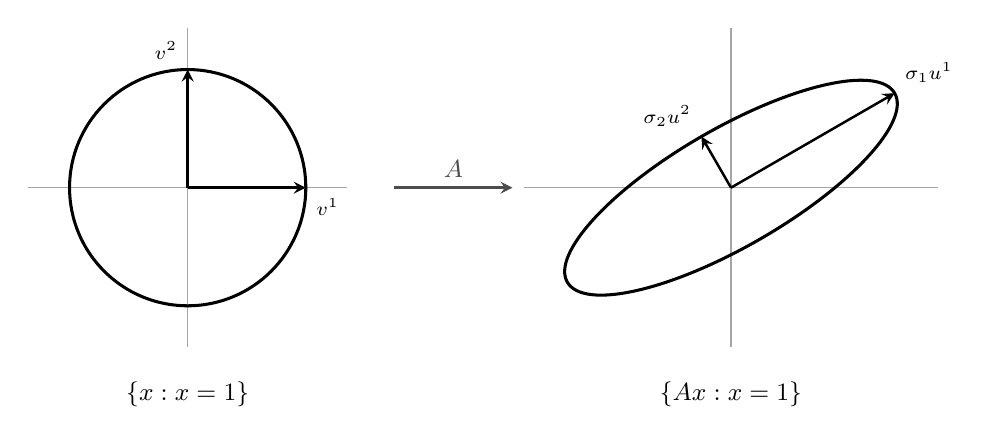
\begin{tikzpicture}[
		scale=1.5,
		>=stealth,
		outline/.style={line width=1.1pt},
		vec/.style={->,line width=0.9pt},
		axisline/.style={line width=0.4pt, black!35},
		maparrow/.style={->,line width=0.9pt,black!70},
	]

	% ---------- domain ----------
	\begin{scope}
		\draw[axisline] (-1.35,0) -- (1.35,0);
		\draw[axisline] (0,-1.35) -- (0,1.35);
		\draw[outline] (0,0) circle (1);
		\draw[vec] (0,0) -- (1,0) node[anchor=north west,font=\scriptsize] {$v^1$};
		\draw[vec] (0,0) -- (0,1) node[anchor=south east,font=\scriptsize] {$v^2$};
		\node[font=\small] at (0,-1.75) {$\{x:\norm{x}=1\}$};
	\end{scope}

	% ---------- the map ----------
	\draw[maparrow] (1.75,0) -- (2.75,0)
	node[midway,above,font=\small] {$A$};

	% ---------- image ----------
	\begin{scope}[shift={(4.6,0)}]
		\draw[axisline] (-1.75,0) -- (1.75,0);
		\draw[axisline] (0,-1.35) -- (0,1.35);
		\draw[outline,rotate=30] (0,0) ellipse [x radius=1.6, y radius=0.5];
		\draw[vec] (0,0) -- (30:1.6)
		node[anchor=south west,font=\scriptsize] {$\sigma_1u^1$};
		\draw[vec] (0,0) -- (120:0.5)
		node[anchor=south east,font=\scriptsize] {$\sigma_2u^2$};
		\node[font=\small] at (0,-1.75) {$\{Ax:\norm{x}=1\}$};
	\end{scope}

\end{tikzpicture}
